\documentclass[12pt]{standalone}
\usepackage{tikz}
\usepackage{anyfontsize}
\begin{document}
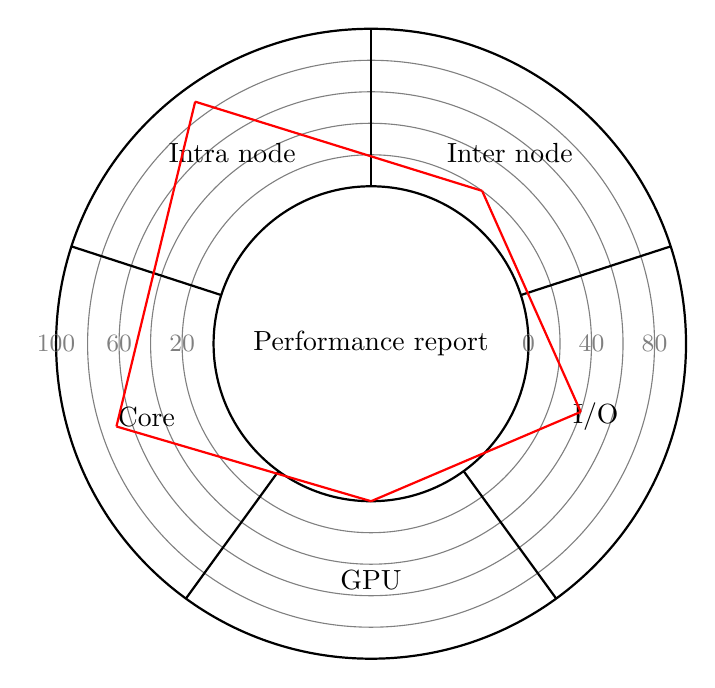
\begin{tikzpicture}
    \draw[thick] (0,0) circle (4.0);
    \draw[gray] (0,0) circle (3.6);
    \draw[gray] (0,0) circle (3.2);
    \draw[gray] (0,0) circle (2.8);
    \draw[gray] (0,0) circle (2.4);
    \draw[thick] (0,0) circle (2.0);
    \foreach \a in {18,90,162,234,306}
        \draw[thick] (\a:2.) -- (\a:4.0);
    \draw (0: 0) node {Performance report};
    \draw (54: 3.0) node {Inter node};
    \draw (126: 3.0) node {Intra node};
    \draw (198: 3.0) node {Core};
    \draw (270: 3.0) node {GPU};
    \draw (342: 3.0) node {I/O};
    \draw[gray, font={\small}] (0: 3.6) node {80};
    \draw[gray, font={\small}] (0: 2.8) node {40};
    \draw[gray, font={\small}] (0: 2.0) node {0};
    \draw[gray, font={\small}] (180: 4.0) node {100};
    \draw[gray, font={\small}] (180: 3.2) node {60};
    \draw[gray, font={\small}] (180: 2.4) node {20};
    \draw[red, thick] (54:2.4)  -- (126:3.8); % end is intra
    \draw[red, thick] (126:3.8) -- (198:3.4); % end is core
    \draw[red, thick] (198:3.4) -- (270:2.0); % end if gpu
    \draw[red, thick] (270:2.0) -- (342:2.8); % 
    \draw[red, thick] (342:2.8) -- (54:2.4);
\end{tikzpicture}
\end{document}
